\section{INTRODUCCIÓN A LOS MÉTODOS DE VECINOS CERCANOS}
    
    Los métodos de Vecinos Cercanos se apoyan en fundamentos matemáticos que deben ser abordados previamente para comprender su funcionamiento de manera profunda. Por esta razón, previo a la explicación de los Métodos de Vecinos Cercanos, se hará una breve introducción a las formas \textit{Representación de Datos} y los métodos de \textit{Medición de Distancias} generalmente usados para implementar ésta técnica.


    \subsubsection{REPRESENTACIÓN DE LOS DATOS}

    A lo largo de este documento se ha hecho uso del concepto de \textit{item} que representa un elemento de recomendación hecho por el sistema.
    Estos items pertenecen a un conjunto de elementos con los que interactúa el usuario y a los que se les pueden describir mediante sus \textit{metadatos}.

    Generalmente, cuando el usuario interactúa con un sistema de recomendación, los items se muestran de forma amigable mediante interfaces que facilitan su interacción. Sin embargo, de forma interna, los algoritmos de recomendación requieren de estructuras de datos que permiten hacer operaciones entre items sin perder sus características únicas. 
    En el caso de los \textit{Métodos de Vecinos Cercanos}, la forma más eficiente de representar la información de cada item es a través de \textbf{vectores}.

    \textbf{VECTORES}

    Un \textit{\textbf{Vector}}, desde un punto de vista geométrico, es un segmento de recta dirigido que corresponde a un desplazamiento entre un punto $A$ y un punto $B$ \parencite{poole2007álgebra}.
    
    Sin embargo, desde el punto de vista algebraico, un vector es definido como un elemento dentro de un \textit{espacio vectorial}.
    
    Los vectores se pueden representar de las siguientes maneras: 

    \begin{equation}
        \addequation{Definición de un Vector (Tupla)}
        \label{vectorTupla}
        \vec{AB} \ = \ (x_1, x_2, \cdots, x_n)
    \end{equation}
    \begin{equation}
        \vec{AB} = 
        \begin{bmatrix}
            x_1
            \\
            x_2
            \\
            \vdots
            \\
            x_n
        \end{bmatrix}
        \addequation{Definición de un Vector (Matriz)}
        \label{vectorMatriz}
    \end{equation}

    Donde la \Cref{vectorTupla} define la representación de un vector mediante tuplas y la \Cref{vectorMatriz} define su representación mediante matrices. Además, es importante puntualizar que cada $x_i$ dentro de un vector es un número real, es decir,  $x_i \in \mathbb{R}$. Por lo tanto, el vector $\vec{AB}$ pertenece al espacio $\mathbb{R}^n$, donde $n$ representa las \textbf{dimensiones} del vector.

    En el contexto de los sistemas de recomendación, los vectores se utilizan para representar de forma algebraica la información numérica de un item. Esto se hace con el propósito de realizar diferentes operaciones algebraicas entre los items para lograr calculos complejos. Además, cuando se habla de vectores que representan items con información extensa se pierde la posibilidad de visualizarlos mediante un plano debido a que las dimensiones suelen crecer en grandes cantidades.

    \newpage

    \subsubsection{MEDICIÓN DE DISTANCIAS}

    Uno de los cálculos más importantes para los sistemas de recomendación es la similitud entre items. Uno de los beneficios de trabajar con vectores es que brindan la posibilidad de usar calculos de medición de distancias que representan de forma numérica la diferencia entre un par de items. Sin embargo, existen diferentes tipos de medición de distancia entre vectores, principalmente la \textit{Distancia Euclidiana}, \textit{Distancia del Coseno} y \textit{Producto Interno}.

    \textbf{DISTANCIA EUCLIDIANA}

    Según \parencite{10.5555/1941884} una de las mediciones de distancia más comunes es la distancia euclideana, que se define mediante la siguiente fórmula:

    \begin{equation}
        d(\vec{x}, \vec{y}) = \sqrt{\sum^n_{k=1}(x_k - y_k)^2}
        \addequation{Definición de Distancia Euclideana}
    \end{equation}

    Donde $\vec{x}, \vec{y} \in \mathbb{R}^n$ o, en otras palabras, el vector $x$ y el vector $y$ pertenecen al mismo campo dimensional $\mathbb{R}^n$. Para expresarlo de manera gráfica, se usará un ejemplo representativo definiendo los siguientes vectores:


    \begin{equation}
        \begin{split}
            &\vec{x} = \begin{bmatrix}
                3
                \\
                5
            \end{bmatrix}, \ 
            \vec{y} = \begin{bmatrix}
                6
                \\
                2
            \end{bmatrix}, \
            (\vec{x}, \vec{y}) \in \mathbb{R}^2
            \\
            \\
            d(\vec{x}, \vec{y}) = &\sqrt{(3 - 6)^2 + (5 - 2)^2} = \sqrt{18} \approx 4.24
        \end{split}
        \addequation{Ejemplo de Distancia Euclidiana}
        \label{EjemploDistanciaEuclidiana}
    \end{equation}

    Como se puede ver en la \Cref{fig: EjemploEuclidiana}, el resultado de la \Cref{EjemploDistanciaEuclidiana} fue aproximadamente igual, por lo tanto, la distancia euclidiana se puede ver graficamente mediante ejemplos representativos como la distancia entre los puntos destino entre dos vectores. Es importante recordar que en el contexto de los sistemas de recomendación el ejemplo dado es un caso excepcional debido a que un item suele estar descrito por más de dos dimensiones.

    \newpage

    \begin{figure}[h!]
        \centering
        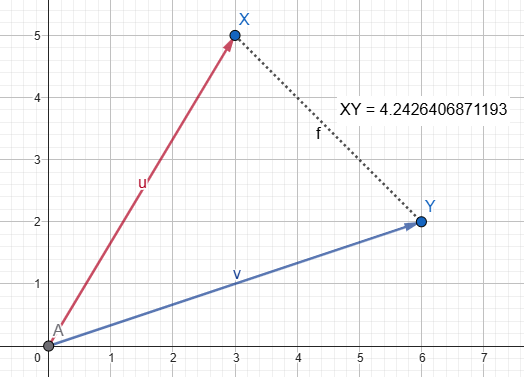
\includegraphics[width=0.8\linewidth]{EjemploEuclidiana.png}
        \caption{Representación gráfica de la Distancia Euclidiana entre dos vectores.}
        \label{fig: EjemploEuclidiana}
    \end{figure}

    \textbf{DISTANCIA DE COSENO}

    Siguiendo a \parencite{10.5555/1941884}, la Distancia del Coseno es otra de las medidas de distancia más comunes cuando un item es considerado un vector. Esta distancia se centra en calcular el coseno del ángulo a través de la \textbf{Similaridad} definida como: 
    
    \begin{equation}
        cos(x, y) = \frac{(\vec{x} \cdot \vec{y})}{|| \ \vec{x} \ || \ || \ \vec{y} \ || }
        \addequation{Definición de la Similaridad de Coseno}
        \label{SimilaridadCoseno}
    \end{equation}

    La fórmula de la Similaridad del Coseno utiliza dos cálculos algebráicos comunes en los vectores, el \textbf{\textit{Producto Punto}} y el calculo de \textbf{\textit{Norma o Magnitud}}.

    Citando a \parencite{poole2007álgebra}, el \textit{Producto Punto} se define como:

    \begin{equation}
        \begin{split}
            \vec{u} = \begin{bmatrix}
                u_1
                \\
                u_2
                \\
                \vdots
                \\
                u_n
            \end{bmatrix} &,  \ \
            \vec{v} = \begin{bmatrix}
                v_1
                \\
                v_2
                \\
                \vdots
                \\
                v_n
            \end{bmatrix}
            \\
            \\
            (u \cdot v) = u_1 v_1 + &u_2 v_2 + \hdots + u_n v_n
        \end{split}
        \addequation{Definición de Producto Punto}
    \end{equation}

    Y la \textit{Norma o Magnitud} de un vector se define como el escalar no negativo $|| \ \vec{v} \ ||$ definido por: 

    \begin{equation}
        \begin{split}
            \vec{V} = &\begin{bmatrix}
                v_1
                \\
                v_2
                \\
                \vdots
                \\
                v_n
            \end{bmatrix}
            \\
            \\
            || \ \vec{V}  \ || = \sqrt{\vec{V} \cdot \vec{V}} &= \sqrt{v_1^2 + v_2^2 + \hdots + v_n^2}
        \end{split}
        \addequation{Definición de Norma o Magnitud}
    \end{equation}    

    Una vez entendiendo cómo calcular la similaridad, se calcula la distancia del coseno:
    
    \begin{equation}
        d(\vec{x}, \vec{y}) = 1 - cos(\vec{x}, \vec{y})
        \addequation{Definición de Distancia del Coseno}
    \end{equation}

    Para ilustrar la distancia del coseno mediante un ejemplo visual se definen los siguientes vectores:

    \begin{equation}
        \begin{split}
            \vec{x} &= \begin{bmatrix}
                3
                \\
                5
            \end{bmatrix},  
            \vec{y} = \begin{bmatrix}
                6
                \\
                2
            \end{bmatrix}
            \\
            \\
            || \vec{x} || &= \sqrt{3^2 + 5^2} = \sqrt{34} \approx 5.83
            \\
            || \vec{y} || &= \sqrt{6^2 + 2^2} = \sqrt{40} \approx 6.32
            \\
            \\
            ( \vec{x} \cdot \vec{y} )&=(3 \cdot  6)+(5 \cdot 2)=28
            \\
            \\
            cos(\vec{x}, \vec{y}) & = \frac{28}{5.83 \cdot 6.32} \approx 0.759
            \\
            \\
            d(\vec{x}, \vec{y}) &\approx 1 - 0.759 \approx  0.241
        \end{split}
        \addequation{Ejemplo de Distancia del Coseno}
        \label{eq:EjemploCoseno}
    \end{equation}

    \newpage

    Para entender las equivalencias entre la \Cref{fig: EjemploCoseno} y la \Cref{eq:EjemploCoseno} es importante mencionar que el calculo geométrico de la Similitud del Coseno se puede realizar mediante el calculo de $cos(\alpha)$ donde $\alpha$ representa el ángulo de separación entre $\vec{x}, \vec{y}$. Entendiendo esto, se puede visualizar que ambos resultados coinciden y representan la distancia del Coseno.

    \begin{figure}[h!]
        \centering
        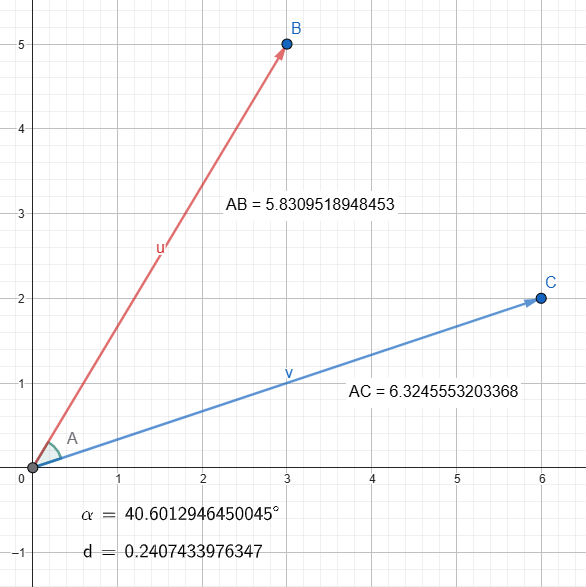
\includegraphics[width=0.8\linewidth]{EjemploCoseno.png}
        \caption{Representación gráfica de la Distancia de Coseno entre dos vectores.}
        \label{fig: EjemploCoseno}
    \end{figure}



    

    \newpage

    





    